%-%-%-%-%-%-%-%-%-%-%-%-%-%-%-%-%-%-%-%-%-%-%-%-%-%-%-%-%-%-%-%-%-%-%-%-%-%-%
%%% MAIN DOCUMENT %%%

%-%-%-%-%-%-%-%-%-%-%-%-%-%-%-%-%-%-%-%-%-%-%-%-%-%-%-%-%-%-%-%-%-%-%-%-%-%-%

\documentclass[12pt, oneside]{book}
\usepackage{xcolor}
\usepackage{minted}

% \usepackage[T1]{fontenc}

\usepackage{draculatheme}
\newcommand{\documentTheme}{draculafg}
\newcommand{\documentLogo}{../../images/small logo_white.png}
\newcommand{\documentBigLogo}{../../images/logo_white_text.png}
\usemintedstyle{dracula}

\usemintedstyle{dracula}

\setminted{
    linenos=true,
    numbersep=5pt,
    frame=lines,
    framesep=2mm,
    breaklines=true
}

% \newcommand{\documentBigLogo}{../../images/Hendrix Logo.png}
% \newcommand{\documentLogo}{../../images/small logo.png}
% \newcommand{\documentTheme}{black}

%%% AESTHETICS %%%
%-%-%-%-%-%-%-%-%-%-%-%-%-%-%-%-%-%-%-%-%-%-%-%-%-%-%-%-%-%-%-%-%-%-%-%-%-%-%


%%% Dimensions and Spacing %%%
\usepackage[margin=1in]{geometry}
\setlength{\parindent}{0pt}
\usepackage{setspace}
\usepackage{mathtools}
\usepackage{esint}
\usepackage{adjustbox}
\linespread{1}
\usepackage{listings}
\usepackage{tikz}
\usetikzlibrary{shapes,backgrounds,calc,patterns,positioning,arrows.meta}
\usepgflibrary{shadings}
\usepackage{pgfkeys}
\usepackage{pdftexcmds}
\usepackage{shellesc}
\usepackage{algorithm, algorithmic, xspace}
%%% Define new colors %%%
\definecolor{orangehdx}{rgb}{0.96, 0.51, 0.16}

% Normal colors
\definecolor{xred}{HTML}{BD4242}
\definecolor{xblue}{HTML}{4268BD}
\definecolor{xgreen}{HTML}{52B256}
\definecolor{xpurple}{HTML}{7F52B2}
\definecolor{xorange}{HTML}{FD9337}
\definecolor{xdotted}{HTML}{999999}
\definecolor{xgray}{HTML}{777777}
\definecolor{xcyan}{HTML}{80F5DC}
\definecolor{xpink}{HTML}{F690EA}
\definecolor{xgrayblue}{HTML}{49B095}
\definecolor{xgraycyan}{HTML}{5AA1B9}

% Dark colors
\colorlet{xdarkred}{red!85!black}
\colorlet{xdarkblue}{xblue!85!black}
\colorlet{xdarkgreen}{xgreen!85!black}
\colorlet{xdarkpurple}{xpurple!85!black}
\colorlet{xdarkorange}{xorange!85!black}
\definecolor{xdarkcyan}{HTML}{008B8B}
\colorlet{xdarkgray}{xgray!85!black}

% Very dark colors
\colorlet{xverydarkblue}{xblue!50!black}

% Document-specific colors
\colorlet{normaltextcolor}{black}
\colorlet{figtextcolor}{xblue}

% Enumerated colors
\colorlet{xcol0}{black}
\colorlet{xcol1}{xred}
\colorlet{xcol2}{xblue}
\colorlet{xcol3}{xgreen}
\colorlet{xcol4}{xpurple}
\colorlet{xcol5}{xorange}
\colorlet{xcol6}{xcyan}
\colorlet{xcol7}{xpink!75!black}

% Blue-Purple (should just used colorbrewer...)
\definecolor{xrainbow0}{HTML}{e41a1c}
\definecolor{xrainbow1}{HTML}{a24057}
\definecolor{xrainbow2}{HTML}{606692}
\definecolor{xrainbow3}{HTML}{3a85a8}
\definecolor{xrainbow4}{HTML}{42977e}
\definecolor{xrainbow5}{HTML}{4aaa54}
\definecolor{xrainbow6}{HTML}{629363}
\definecolor{xrainbow7}{HTML}{7e6e85}
\definecolor{xrainbow8}{HTML}{9c509b}
\definecolor{xrainbow9}{HTML}{c4625d}
\definecolor{xrainbow10}{HTML}{eb751f}
\definecolor{xrainbow11}{HTML}{ff9709}

%------- %
% XHFILL %
%------- %



%%% Chapter Headings %%%

\newcommand{\gradientrule}{
    \begin{tikzpicture}
        \shade[left color=orangehdx, right color=black, middle color=gray] (0,0) rectangle (\linewidth,0.4pt);
    \end{tikzpicture}
}

\usepackage[Glenn]{fncychap}
\ChTitleVar{\bfseries\scshape\color{\documentTheme}} % Needed for Dracula theme
\ChNumVar{\large\selectfont\color{\documentTheme}} % Needed for Dracula theme
\ChNameVar{\large\color{\documentTheme}} % Needed for Dracula theme
\usepackage{xpatch}


\xpatchcmd\DOCH
{\mghrulefill}{\color{orangehdx}\mghrulefill}
{}{\PatchFailed}
\xpatchcmd\DOTI
{\mghrulefill}{\color{orangehdx}\mghrulefill}
{}{\PatchFailed}
\xpatchcmd\DOTIS
{\mghrulefill}{\color{orangehdx}\mghrulefill}
{}{\PatchFailed}



%% Change Chapter Heading Placement %%
\usepackage{etoolbox}
\makeatletter
\patchcmd{\@makechapterhead}{\vspace*{50\p@}}{\vspace*{-20\p@}}{}{}
\patchcmd{\@makeschapterhead}{\vspace*{50\p@}}{\vspace*{-20\p@}}{}{}
\patchcmd{\DOTI}{\vskip 80\p@}{\vskip 40\p@}{}{}
\patchcmd{\DOTIS}{\vskip 40\p@}{\vskip 0\p@}{}{}
\makeatother



\renewcommand{\thesection}{\thechapter.\arabic{section}} %% Chapter.Section Numbering


%%% listingS %%%
\usepackage{graphicx}  
% \numberwithin{listing}{section}
\usepackage{float}
\usepackage{caption}

%%% Hyperlinks %%%
\usepackage{hyperref}
\definecolor{horange}{HTML}{f58026}
\hypersetup{
	colorlinks=true,
	linkcolor=horange,
	filecolor=horange,      
	urlcolor=horange,
}

\newcommand{\assignmentname}{Homework 7: Chapter 8}

%% Headers and Footers %%
\usepackage{fancyhdr} % This should be set AFTER setting up the page geometry
\pagestyle{fancy} % options: empty , plain , fancy
\fancyhead[R]{\textcolor{draculafg}{\assignmentname}}
\fancyhead[L]{\textcolor{draculafg}{Hendrix College}}
\fancyhead[C]{\includegraphics[height=.50cm]{\documentLogo}} % Use for Dracula
\usepackage{xpatch}
\xpretocmd\headrule{\color{orangehdx}}{}{\PatchFailed}
\setlength{\footskip}{0.5in}
\setlength{\headheight}{18.5764pt}


%%%%% Colored Boxes %%%%%
\usepackage{tcolorbox}
\tcbuselibrary{skins}
\tcbuselibrary{theorems}
% \tcbuselibrary{minted}
\newcounter{BoxCounter}
\usepackage{dingbat}

%-%-%-%-%-%-%-%-%-%-%-%-%-%-%-%-%-%-%-%-%-%-%-%-%-%-%-%-%-%-%-%-%-%-%-%-%-%-%

%% MATH PACKAGES, ENVIRONMENTS, COMMANDS %%
%-%-%-%-%-%-%-%-%-%-%-%-%-%-%-%-%-%-%-%-%-%-%-%-%-%-%-%-%-%-%-%-%-%-%-%-%-%-%
%You'll need your own packages, theorem types, and commands.

\usepackage{fix-cm}
\usepackage{amsmath,amsthm} 
\usepackage{array, makecell}
\usepackage{colortbl}
\newcommand{\thickvrule}{\vrule width 1pt}

\newcommand{\thickhrule}{\Xhline{1pt}}

\usepackage{mathtools}
\usepackage{amssymb}
\usepackage[framemethod=tikz]{mdframed}
\usepackage{mathrsfs}
\usepackage{changepage}
\usepackage{multicol}
\usepackage{slashed}
\usepackage{enumerate}
\usepackage{braket}
\usepackage{booktabs}
\usepackage{enumitem}
\usepackage{kantlipsum}  %This package lets us generate random text for example purposes.
\usepackage{pgfplots}


%%% Custom Commands %%%
% Natural Numbers 
\newcommand{\N}{\mathbb{N}}

% Whole Numbers
\newcommand{\W}{\mathbb{W}}

% Integers
\newcommand{\Z}{\mathbb{Z}}

% Rational Numbers
\newcommand{\Q}{\mathbb{Q}}

% Real Numbers
\newcommand{\R}{\mathbb{R}}

% Complex Numbers
\newcommand{\C}{\mathbb{C}}

\newcommand{\I}{\mathbb{I}}

\newcommand{\pfs}{\noindent\makebox[\linewidth]{\rule{\textwidth}{0.4pt}}\vspace{0.5cm}}

\newcommand{\mysqrt}[1]{%
	\mathpalette\foo{#1}%
}
\newcommand{\dmysqrt}[1]{%
	\mathpalette\foodisplay{#1}%
}

% !TeX spellcheck = off
\newcommand{\foo}[2]{%
	% #1: math style, #2: content
	\sbox0{$#1\sqrt{#2}$}% Measure the size of the standard sqrt in the current style
	\begin{tikzpicture}[baseline=(sqrt.base)]
		\node[inner sep=0, outer sep=0] (sqrt) {$#1\sqrt{#2}$}; % Use the current math style
		\draw([yshift=-0.045em]sqrt.north east) -- ++(0,-0.5ex); % Draw the tick
	\end{tikzpicture}%
}
% !TeX spellcheck = off
\newcommand{\foodisplay}[2]{%
	% #1: math style, #2: content
	\sbox0{$#1\sqrt{#2}$}% Measure the size of the standard sqrt in the current style
	\begin{tikzpicture}[baseline=(sqrt.base)]
		\node[inner sep=0, outer sep=0] (sqrt) {$\displaystyle\sqrt{#2}$}; % Force displaystyle
		\draw[line width=0.4pt] ([yshift=-0.044em]sqrt.north east) -- ++(0,-0.5ex); % Draw the tick
	\end{tikzpicture}%
}

\renewcommand{\theenumi}{\arabic{enumi}}
\renewcommand{\labelenumi}{\textbf{\theenumi}.}
\renewcommand{\theenumii}{\alph{enumii}}
\renewcommand{\labelenumii}{\textbf{\theenumii}.}

% \newcommand{}{\marginnote{
\includegraphics[width=2em]{caution.png}}}

\newmdenv[
	topline=false,
	bottomline=true,
	rightline=false,
	leftline=true,
	linewidth=1.5pt,
	linecolor=black, % default color, will be overridden in custom commands
	backgroundcolor=draculabg, % Needed for Dracula theme
	fontcolor=\documentTheme, % Needed for Dracula theme
	innertopmargin=0pt,
	innerbottommargin=5pt,
	innerrightmargin=10pt,
	innerleftmargin=10pt,
	leftmargin=0pt,
	rightmargin=0pt,
	skipabove=\topsep,
	skipbelow=\topsep,
]{customframedproof}

\newenvironment{proofpart}[2][black]{
    \begin{mdframed}[
        topline=false,
        bottomline=false,
        rightline=false,
        leftline=true,
        linewidth=1pt,
        linecolor=#1!40, % Custom color
        % innertopmargin=10pt,
        % innerbottommargin=10pt,
        innerleftmargin=10pt,
        innerrightmargin=10pt,
        leftmargin=0pt,
        rightmargin=0pt,
        % skipabove=\topsep,
        % skipbelow=\topsep%
    ]
    \noindent
    \begin{minipage}[t]{0.08\textwidth}%
        \textbf{#2}%
    \end{minipage}%
    \begin{minipage}[t]{0.90\textwidth}%
        \begin{adjustwidth}{0pt}{0pt}%
}{
    \end{adjustwidth}
    \end{minipage}
    \end{mdframed}
}

% Define a new environment 'proofscratch' for Proof and Scratch Paper
\newenvironment{proofscratch}[2]{%
    \begin{mdframed}[
        topline=false,
        bottomline=false,
        rightline=false,
        leftline=false,
        backgroundcolor=draculabg, % Background color for Dracula theme
        fontcolor=\documentTheme,       % Font color for Dracula theme
        innerleftmargin=-6pt,
        innertopmargin=0pt,
        leftmargin=0pt,
        rightmargin=0pt,
        skipabove=\topsep,
        skipbelow=\topsep,
    ]
    % % Begin TikZ picture for the vertical dotted line
    % \begin{tikzpicture}[overlay, remember picture]
    %     % Draw a vertical dotted line at approximately the center of the mdframed width
    %     \draw[dotted, thick] ([xshift=0.005\linewidth]current bounding box.north west) -- ([xshift=0.005\linewidth]current bounding box.south west);
    % \end{tikzpicture}%
    % % Create the left minipage for Proof
    \begin{minipage}[t]{0.47\textwidth}%
        \noindent\textit{Proof.} #1 \hfill \(\qed\)
    \end{minipage}%
    \hfill
    % Create the right minipage for Scratch Paper
    \begin{minipage}[t]{0.47\textwidth}%
        \textit{Scratch Paper.} #2
    \end{minipage}%
}{
    \end{mdframed}
}

\newenvironment{tipbox}
	{%
		\par\noindent%
		% Top dashed line (using \textwidth)
		\tikz[baseline]{\draw[dash pattern=on 3pt off 2pt, line width=0.5pt, color=draculapurple] (0,0) -- (\textwidth,0);}%
		\par\vspace{0.65em}%
		\noindent\textbf{\textcolor{draculapurple}{TIP:}}\quad%
	}
	{%
		\par%
		% Bottom dashed line
		\noindent%
		\tikz[baseline]{\draw[dash pattern=on 3pt off 2pt, line width=0.5pt, color=draculapurple] (0,0) -- (\textwidth,0);}%
		\par\vspace{0.35em}
	}

\newenvironment{notebox}
	{%
		\par\noindent%
		% Top dashed line (using \textwidth)
		\tikz[baseline]{\draw[dash pattern=on 3pt off 2pt, line width=0.5pt, color=draculagreen] (0,0) -- (\textwidth,0);}%
		\par\vspace{0.65em}%
		\noindent\textbf{\textcolor{draculagreen}{NOTE:}}\quad%
	}
	{%
		\par%
		% Bottom dashed line
		\noindent%
		\tikz[baseline]{\draw[dash pattern=on 3pt off 2pt, line width=0.5pt, color=draculagreen] (0,0) -- (\textwidth,0);}%
		\par\vspace{0.35em}
	}

\newenvironment{warningbox}
	{%
		\par\noindent%
		% Top dashed line (using \textwidth)
		\tikz[baseline]{\draw[dash pattern=on 3pt off 2pt, line width=0.5pt, color=draculared] (0,0) -- (\textwidth,0);}%
		\par\vspace{0.65em}%
		\noindent\textbf{\textcolor{draculared}{WARNING:}}\quad%
	}
	{%
		\par%
		% Bottom dashed line
		\noindent%
		\tikz[baseline]{\draw[dash pattern=on 3pt off 2pt, line width=0.5pt, color=draculared] (0,0) -- (\textwidth,0);}%
		\par\vspace{0.35em}
	}

\newenvironment{solution}{\textit{Solution.}}

\newcommand{\sol}[1]{
    \begin{customframedproof}[linecolor=orangehdx!75,]
        \begin{solution}
        #1
        \end{solution}
    \end{customframedproof}
}

\newcommand{\pf}[1]{
    \begin{customframedproof}[linecolor=orangehdx!75]
        \begin{proof}
        #1
        \end{proof}
    \end{customframedproof}
}

\def \proofDistance {10pt}

\newcommand{\disabs}[1]{\ensuremath{\left|#1\right|}}
\newcommand{\limn}{\lim_{n \rightarrow \infty}}
\newcommand{\limx}[2]{\lim_{x \rightarrow #1}#2}

\newcommand{\limc}[1]{\lim_{x \rightarrow c}#1}

\newcommand{\ninn}{n \in \N}

\newcommand{\mb}[1]{\mathbf{#1}}

\newcommand{\limsupn}[1]{\limsup_{n\rightarrow \infty}#1}
\newcommand{\liminfn}[1]{\liminf_{n\rightarrow \infty}#1}


\newcommand{\proj}{\text{proj}}

\newcommand{\p}{\partial}

\newcommand{\dydx}{\frac{dy}{dx}}
\newcommand{\dxdy}{\frac{dx}{dy}}
\newcommand{\dydt}{\frac{dy}{dt}}
\newcommand{\dxdt}{\frac{dx}{dt}}
\newcommand{\dzdt}{\frac{dz}{dt}}

\newcommand{\barNotationT}[1]{\bigg|_{t = #1}}

\newcommand{\cyanit}[1]{\textit{\textcolor{cyan}{#1}}}

\newcommand{\brackett}[1]{\left\langle #1 \right\rangle}

\newcommand{\norm}[1]{\left\lVert \mathbf{#1}\right\rVert}

\newcommand{\imb}{\mb{i}}
\newcommand{\jmb}{\mb{j}}
\newcommand{\kmb}{\mb{k}}
\newcommand{\rmb}{\mb{r}}
\newcommand{\umb}{\mb{u}}

\newcommand{\vecfuc}[2]{\mb{#1}(#2)}
\newcommand{\dvecfuc}[2]{\mb{#1}'(#2)}
\newcommand{\normdvecfuc}[2]{\|\mb{#1}'(#2)\|}

\newcommand{\squigglyline}{%
    \noindent
    \tikz[baseline=-0.5ex]{
        \draw[decorate, decoration={snake, amplitude=0.5mm, segment length=3mm}] 
        (0,0) -- (\dimexpr\linewidth\relax,0);
    }%
}


% end of preamble
%-%-%-%-%-%-%-%-%-%-%-%-%-%-%-%-%-%-%-%-%-%-%-%-%-%-%-%-%-%-%-%-%-%-%-%-%-%-%

\begin{document}


%-%-%-%-%-%-%-%-%-%-%-%-%-%-%-%-%-%-%-%-%-%-%-%-%-%-%-%-%-%-%-%-%-%-%-%-%-%-%
%%% COVER PAGE %%%
%-%-%-%-%-%-%-%-%-%-%-%-%-%-%-%-%-%-%-%-%-%-%-%-%-%-%-%-%-%-%-%-%-%-%-%-%-%-%

% Do not use all caps.
\newcommand{\cussubtitle}{Mathematical Models}
% Date format should be like: "January 1, 2001"
\newcommand{\finaldate}{April 21, 2026}
% Be sure to include degree recognition (e.g., B.S., M.S., Ph.D)
\newcommand{\professor}{Dr. Christopher Camfield}

% -%-%-%-%-%-%-%-%-%-%-%-%-%-%-%-%-%-%-%-%-%-%-%-%-%-%-%-%-%-%-%-%-%-%-%-%-%-%

\begin{titlepage}
    \begin{center}

        \vspace*{-2cm}
        \includegraphics[width=0.8\textwidth]{\documentBigLogo}\\
        \vfill

        % Horizontal line above the title in 'horange' color
        \textcolor{horange}{\rule{\textwidth}{1.0pt}}

        \vspace{2em}

        {\huge \textbf{\assignmentname}}

        \vspace{1em} % Space between the title and the bottom line

        \textcolor{horange}{\rule{\textwidth}{1.0pt}}

        \vspace*{1\baselineskip}

        {\LARGE \textbf{\cussubtitle}}

        \begin{large}
            \vspace*{5\baselineskip}

            \vspace*{1\baselineskip}

            \emph{Author} \\[1ex]
            %Submitted by \\[\baselineskip]
            {\Large Paul Beggs \\ \par} % Editor list
            {\href{mailto:BeggsPA@Hendrix.edu}{{BeggsPA@Hendrix.edu}}}\\ % Editor affiliation

            \vspace*{1\baselineskip}

            \textit{Instructor} \\[1ex] % Tagline(s) or further description
            \professor

            \vspace*{1\baselineskip}

            \textit{Due}\\[1ex]
            {\scshape  \finaldate} \\[0.3\baselineskip] % Year published

            \thispagestyle{empty}

        \end{large}
    \end{center}
\end{titlepage}
% -%-%-%-%-%-%-%-%-%-%-%-%-%-%-%-%-%-%-%-%-%-%-%-%-%-%-%-%-%-%-%-%-%-%-%-%-%-%


\section*{Chapter 8}

% Chapter 8, Exercise 3
% Chapter 8, Exercise 6
% Chapter 8, Exercise 8

\begin{enumerate}
    \setcounter{enumi}{2}
    \item Reconsider the inventory problem of Example 8.1, but now suppose that the inventory policy depends on recent sales history. Whenever inventory drops to zero, the number of units ordered is equal to two plus the number sold over the past week, up to a maximum of four.
    \begin{enumerate}
        \item Determine the steady–state probability distribution of the number of aquariums in stock. Use the five-step method, and model as a Markov chain.
        \sol{
            With transition matrix
            \[
                P = \begin{pmatrix}
                    0.368 & 0 & 0.632 & 0 \\
                    0.368 & 0.368 & 0 & 0.264 \\
                    0.184 & 0.368 & 0.368 & 0.080 \\
                    0.061 & 0.184 & 0.368 & 0.387 
                \end{pmatrix},
            \]
            we find the steady-state probability distribution of the number of aquariums in stock to be \(\pi = [0.258, 0.245, 0.346, 0.151]\).
        }
        \item Determine the steady–state probability that demand exceeds supply.
        \sol{
            Our goal is to find 
            \[
                \sum_{i = 1}^{4}P(X_{n} = i)P(D_{n} > i),
            \]
            where \(P(X_{n} = i)\) is \(\pi_{i}\) such that \(i\) corresponds to an index in \(\pi\). We find \(P(D_{n} > i)\) by the complement rule:
            \[
                P(D_{n} > i) = 1 - P(D_{n} \le i).
            \]
            By this procedure, we find the probability that demands exceeds supply to be \(9.5\)\%. 
        }
        \item Determine the average size of a resupply order.
        \sol{
            From the reordering rule, we know that we will never receive more than 4 aquariums per order. If we sell out, then we add what we sold plus 2 to the order. Thus, if \(X_{n} = 1\) and the demand is 1, then the order is 3. Following the same pattern (and adhering to the restocking policy), we find that when \(X_{n} = 2\), 3 or 4, the order is 4. To find the average order per week, we sum the probability of triggering an order from each state, multiplied by the order size for that state:
            \[
                E[\text{Volume}] = \sum_{i = 1}^{4} \pi_{i} \cdot P(D \ge i) \cdot (\text{Order Size}_{i}).
            \]
            This yields approximately 0.870 aquariums per week. To find the average aquariums on a per-order basis, we need to find the average order size given there is an order placed. That is,
            \[
                E[\text{Order Size} \mid \text{Order Placed}] = \frac{E[\text{Volume}]}{ P(\text{Order})}.
            \]
            We find the probability of placing an order by summing the probabilities of selling out:
            \[
                P(\text{Order}) = \sum_{i = 1}^{4} \pi_{i}P(D \ge i) = 0.259
            \]
            Thus, we find the average order to be 3.37 aquariums per week.

        }
        \item Repeat parts (a) and (b), but now suppose that weekly demand is Poisson with a mean of 2 customers per week.
        \sol{
            For \(\lambda = 2\), we get steady state \([0.215, 0.187, 0.306, 0.291]\) for aquariums in stock, and we find the steady state probability that demand exceeds supply to be 24.7\%.
        }
    \end{enumerate}

\hfill
\begin{figure}[h]
    \label{fig:trans dia E6}
    \centering
    \begin{tikzpicture}[
        >=Stealth, % sets arrowhead style
        every path/.style={->, thick}, % applies to all arrows
    ]
        % Nodes
        \node[draw, circle, inner sep=7pt] (A) at (0,0) {4};
        \node[draw, circle, inner sep=7pt] (B) at (8,0) {3};
        \node[draw, circle, inner sep=7pt] (C) at (8,8) {2};
        \node[draw, circle, inner sep=7pt] (D) at (0,8) {1};
        \node[draw, circle, inner sep=7pt] (E) at (4,4) {0};
        
        % State 0 to all other states:
        \draw (E) to[out=180, in=270, looseness=1]
            node[midway, below left] {0.05} (D);

        \draw (E) to[out=170, in=130, looseness=4]
            node[midway, above left] {0.9} (E);

        \draw (E) to[out=90, in=180, looseness=1]
            node[midway, above left] {0.025} (C);

        \draw (E) to[out=0, in=90, looseness=1]
            node[midway, below left] {0.015} (B);

        \draw (E) to[out=270, in=0, looseness=1]
            node[midway, above left] {0.01} (A);

        % State 1 to all other states:
        \draw (D) to[out=0, in=100, looseness=1]
            node[midway, below left] {0.3} (E);
        
        \draw (D) to[out=170, in=130, looseness=4]
            node[midway, above left] {0.7} (D);

        % State 2 to all other states:
        \draw (C) to[out=170, in=10, looseness=1]
            node[midway, above] {0.4} (D);
        
        \draw (C) to[out=80, in=40, looseness=4]
            node[midway, above right] {0.6} (C);

        % State 3 to all other states:
        \draw (B) to[out=80, in=280, looseness=1]
            node[midway, right] {0.6} (C);
        
        \draw (B) to[out=350, in=310, looseness=4]
            node[midway, below right] {0.4} (B);

        % State 4 to all other states:
        \draw (A) to[out=350, in=190, looseness=1]
            node[midway, below] {0.8} (B);
        
        \draw (A) to[out=260, in=220, looseness=4]
            node[midway, below left] {0.2} (A);


    \end{tikzpicture}
    \caption{State transition probability diagram for Exercise 6, part (a).}
\end{figure}

        \setcounter{enumi}{5}
\newpage

        \item A Markov chain model of floods uses the state variable \(X_{n} = 0, 1,2,3,4\) where state 0 means the average daily flow is below 1,000 cubic feet per second, state 1 is 1,000--2,000 cfs, state 2 is 2,000--5,000 cfs, 3 is 5,000--10,000 cfs, and 4 is over 10,000 cfs. The state transition probability matrix for this model is
        \[
            P = \begin{pmatrix}
                0.9 & 0.05 & 0.025 & 0.015 & 0.01 \\
                0.3 & 0.7 & 0 & 0 & 0 \\
                0 & 0.4 & 0.6 & 0 & 0 \\
                0 & 0 & 0.6 & 0.4 & 0 \\
                0 & 0 & 0 & 0.8 & 0.2
            \end{pmatrix}
        \]
        \begin{enumerate}
            \item Draw the state transition probability diagram for this model.
            \sol{
                The diagram for this model is presented in \hyperref[fig:trans dia E6]{Figure 1}.
            }
            \item Find the steady–state probability distribution for this model.
            \sol{
                The steady-state probability distribution for this model is \(\pi = [0.661, 0.22, 0.083, 0.028, 0.008]\).
            }
            \item How often are severe floods (over 10,000 cfs) expected to occur?
            \sol{
                Over \(N\) days, the river spends around \(N\pi_{4}\) days in state 4. Thus, the average gap between consecutive days is \(N/(N\pi_{4}) = 1/\pi_{4} = 121\) days.
            }
            \item A reservoir used for drought storage depends on the flow of this river. When the flow is over 5,000 cfs, the reservoir is allowed to store 1,000 acre--feet per day. When the flow is under 1,000 cfs, the reservoir is required to release 100 acre--feet per day back into the river. Find the expected annual number of acre--feet of water stored in the reservoir. Is this number positive or negative? What does this mean?
            \sol{
                To find the expected annual number of acre--ft of water stored in the reservoir, we calculate
                \[
                    365(- \pi_{0}100 + 1000(\pi_{3} + \pi_{4})) = -11060.61.
                \]
                This number is negative, which implies there is not enough water to be put back into river when it is needed.
            }
        \end{enumerate}


\newpage

    \setcounter{enumi}{7}



    \item Reconsider the forklift problem of Example 8.3, but now suppose that a second mechanic is called in whenever two or more trucks need repair.
    \begin{enumerate}
        \item Determine the steady–state distribution of the number of trucks needing repair. Use the five-step method and model as a Markov process.
        \sol{
            The change with scheduling suggests a new flow matrix of
            \[
                \begin{pmatrix}
                    -\lambda & \mu & 0 & 0 & \cdots & 0 & 0 \\
                    \lambda & -(\lambda + \mu) & 2\mu & 0 & \cdots & 0 & 0 \\
                    0 & \lambda & -(\lambda + 2\mu) & 2\mu & \cdots & 0 & 0 \\
                    \vdots & \vdots & \vdots & \vdots & \ddots & \vdots & \vdots \\
                    0 & 0 & 0 & 0 & \cdots & \lambda & -2\mu
                \end{pmatrix},
            \]
            where the `\(\cdots\)' represent 23 columns of zeros. With this change, we find 
            \begin{multline*}
                \pi = [0.53043, 0.32549, 0.09987, 0.03064, 0.0094, 0.00288, 0.00089,\\
                0.00027, 8 \times 10^{-5}, 3 \times 10^{-5}, 1 \times 10^{-5}, 0, \ldots, 0],
            \end{multline*}
            where also for \(i \ge 11\), \(\pi_{i}= 0\). 
        }
        \item Use the results of part (a) to calculate the steady--state expected number of forklift trucks in the repair facility, the probability that the first mechanic is busy, and the probability that the second mechanic is called in. Compare to the results obtained for one mechanic in Example 8.3.
        \sol{
            We would expect 0.68 trucks in the repair facility on an average day. By solving \(P(X_{t} > 0) = 1 - P(X_{t} = 0) = 1 - \pi_{0}\), we find that the first mechanic is busy only 47.0\% of the time. Similarly, by solving \(P(X_{t} \ge 2) = 1 - (P(X_{t} = 0) + P(X_{t} = 1))\), we find the second mechanic is called in 14.4\% of the time. 
            
            Compared to when we just had one mechanic, we see that the number of trucks in the facility has been cut by over half. That is, there is a \(1.607 - 0.68 = 0.927\) reduction in trucks in the workshop on any given day. 
            
            We also see that the first mechanic is working less now than what they were, with a \(61.4\% - 47\% = 14.4\%\) difference (which \textit{conveniently} matches the time the second mechanic is called in). 
            
            In conclusion, there are less trucks sitting in the repair shop at any given time, even though the first mechanic is working less. This implies that the second mechanic coming in only 14.4\% of the time is really making a huge difference on overall productivity.

            That is, by hiring the second mechanic, they have cut the time trucks sit idle in the shop by \(0.927/1.607 = 57.7\%\).
        }

\newpage


        \item The cost of the second mechanic is \$250 per day, and the mechanic is only paid for the days worked. Another option which can be used in case of backlog (two or more trucks in repair) is to lease replacement vehicles for customers whose trucks are in repair, at a cost of \$125 per week per vehicle. Which of the two plans is most cost-effective?
        \sol{
            We find the first option of hiring another mechanic has a lower yearly cost of \(\$10323.32 - \$9508.70 = \$814.62\) per year. We get the cost of paying a mechanic by using the probability of one being called multiplied the product of yearly working days and the daily rate. That is,
            \[
                0.14407 \times 12 \times 22 \times \$250 = \$\text{9,508.70}.
            \]
            We find the yearly cost of leasing vehicles by using Example 8.3's steady-state distribution, \(\hat{\pi}\). In that, we multiply the total number of weeks in a year by the product of the sum of the expected number of trucks that are in repair at any given time and \$125. That is,
            \[
                52 \times \left(\sum_{i = 1}^{27} i \times \hat{\pi}_{i}\right) \times \$125 = \$\text{10,323.32}.
            \]
            If the intention of the leasing option is to not include leasing the truck that is being actively repaired (i.e., \(i\) starts at 2 instead of 1), then leasing would actually be better. It would have a cost-saving margin of \$726.45 dollars per year.
        }

        \item  There is some uncertainty as to the actual cost of bringing in a second mechanic during periods of backlog. What is the minimum cost per day for a second mechanic that makes leasing a better alternative?
        \sol{
            To find the minimum cost \(x\) that makes leasing a better alternative, we solve for \(x\) in
            \[
                38.03448x = 10323.32,
            \]
            and find the minimum cost per day to be \$271.42 for the leasing option to break even with the cost of hiring the second mechanic.
        }

    \end{enumerate}
\end{enumerate}





\end{document}